\documentclass{InsightArticle}

\usepackage[dvips]{graphicx}
\usepackage{float}
\usepackage{subfigure}

\usepackage[dvips,
bookmarks,
bookmarksopen,
backref,
colorlinks,linkcolor={blue},citecolor={blue},urlcolor={blue},
]{hyperref}

\title{Interactive Correspondence Selection}

% 
% NOTE: This is the last number of the "handle" URL that 
% The Insight Journal assigns to your paper as part of the
% submission process. Please replace the number "1338" with
% the actual handle number that you get assigned.
%
\newcommand{\IJhandlerIDnumber}{3313}

% Increment the release number whenever significant changes are made.
% The author and/or editor can define 'significant' however they like.
\release{0.00}

% At minimum, give your name and an email address.  You can include a
% snail-mail address if you like.

\author{David Doria}
\authoraddress{Rensselaer Polytechnic Institute, Troy NY}


\begin{document}

\IJhandlefooter{\IJhandlerIDnumber}


\ifpdf
\else
   %
   % Commands for including Graphics when using latex
   % 
   \DeclareGraphicsExtensions{.eps,.jpg,.gif,.tiff,.bmp,.png}
   \DeclareGraphicsRule{.jpg}{eps}{.jpg.bb}{`convert #1 eps:-}
   \DeclareGraphicsRule{.gif}{eps}{.gif.bb}{`convert #1 eps:-}
   \DeclareGraphicsRule{.tiff}{eps}{.tiff.bb}{`convert #1 eps:-}
   \DeclareGraphicsRule{.bmp}{eps}{.bmp.bb}{`convert #1 eps:-}
   \DeclareGraphicsRule{.png}{eps}{.png.bb}{`convert #1 eps:-}
\fi


\maketitle


\ifhtml
\chapter*{Front Matter\label{front}}
\fi

\begin{abstract}
\noindent
This document presents a GUI application to manually select corresponding points in two data sets. The data sets can each be either an image or a point cloud. If both data sets are images, the functionality is equivalent to Matlab's 'cpselect' function. There are many uses of selecting correspondences. If both data sets are images, the correspondences can be used to compute the fundamental matrix, or to perform registration. If both data sets are point clouds, the correspondences can be used to compute a landmark transformation. If one data set is an image and the other is a point cloud, the camera matrix relating the two can be computed.

\end{abstract}

\IJhandlenote{\IJhandlerIDnumber}

\tableofcontents
\section{Introduction}
This document presents a GUI application to manually select corresponding points in two data sets. The data sets can each be either an image or a point cloud. If both data sets are images, the functionality is equivalent to Matlab's 'cpselect' function. There are many uses of selecting correspondences. If both data sets are images, the correspondences can be used to compute the fundamental matrix, or to perform registration. If both data sets are point clouds, the correspondences can be used to compute a landmark transformation. If one data set is an image and the other is a point cloud, the camera matrix relating the two can be computed.

%%%%%%%%%%%%%%%%
\section{GUI}
\label{sec:GUI}

The GUI is divided into a left pane and a right pane. Either type of data set (image or point cloud) can be loaded in either pane. Figure \ref{fig:GUI} shows the GUI with an image loaded in the left pane and a point cloud loaded in the right pane.

\begin{center}
  \begin{figure}[H]
  \centering
    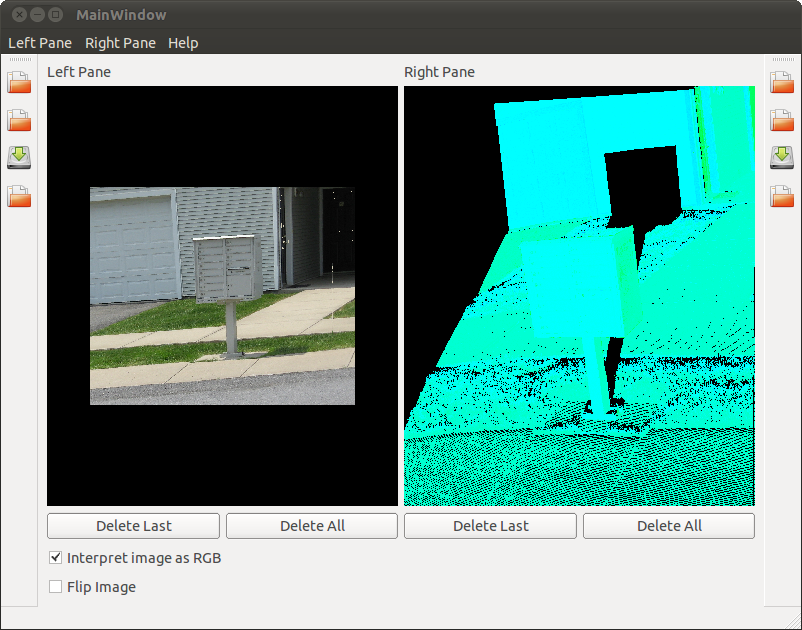
\includegraphics[width=0.6\linewidth]{images/GUI}
    \caption{Screenshot of the GUI}
    \label{fig:GUI}
  \end{figure}
\end{center} 

There is a toolbar for each pane with all of the possible actions that can be taken (load an image, load a point cloud, save correspondences, and load correspondences). These actions are also available from the file menu corresponding to each pane.

%%%%%%%%%%%%%%%%
\section{Correspondence Selection}
The correspondence selection is slightly different in images and point clouds.

\subsection{Image Correspondence Selection}
The interaction in image mode is done using a vtkInteractorStyleImage. Therefore, the controls are:
\begin{itemize}
 \item Hold the right mouse button and drag to zoom in and out.
 \item Hold the middle mouse button and drag to pan the image.
\end{itemize}

Correspondences are then selected using the left mouse button.

Both a vtkCaptionActor2D and a red sphere are drawn to indicate the position of the correspondence. When zoomed out, the vtkCaptionActor2D indicates the general position of the point, as shown in Figure \ref{fig:ImageZoomedOut}.
\begin{center}
  \begin{figure}[H]
  \centering
    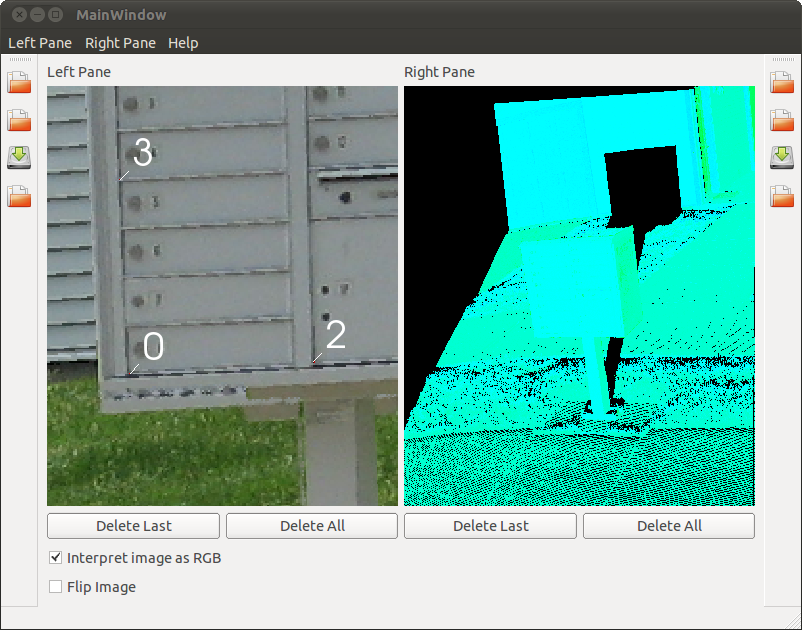
\includegraphics[width=0.6\linewidth]{images/ImageZoomedOut}
    \caption{Screenshot of a zoomed out view of image correspondences}
    \label{fig:ImageZoomedOut}
  \end{figure}
\end{center} 

When zoomed in, the sphere indicates the exact position of the point, as shown in Figure \ref{fig:ImageZoomedIn}. The sphere has radius 0.5, so it is the size of one pixel.

\begin{center}
  \begin{figure}[H]
  \centering
    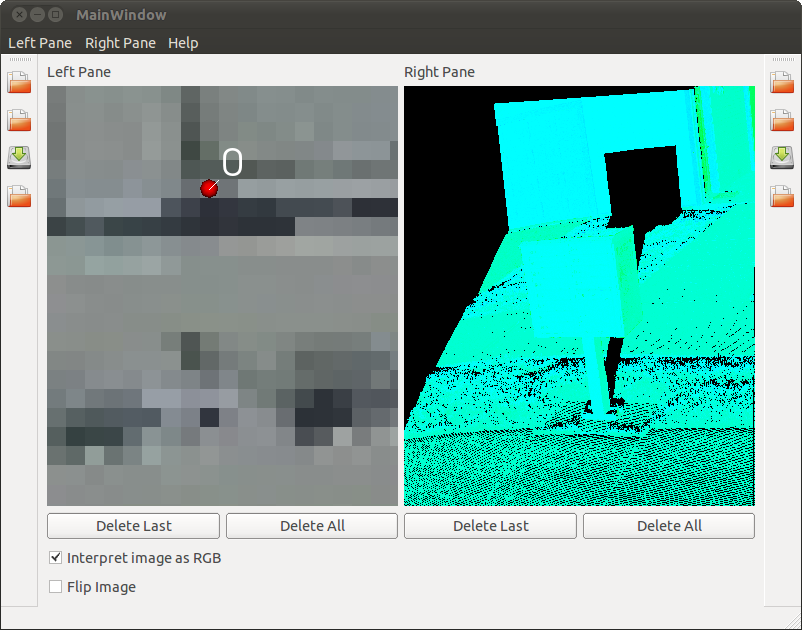
\includegraphics[width=0.6\linewidth]{images/ImageZoomedIn}
    \caption{Screenshot of a zoomed in view of image correspondences}
    \label{fig:ImageZoomedIn}
  \end{figure}
\end{center} 

\subsection{Point Cloud Correspondence Selection}
The interaction in point cloud mode is done using a vtkInteractorStyleTrackballCamera. Therefore, the controls are:
\begin{itemize}
 \item Hold the left mouse button and drag to rotate the scene.
 \item Hold the right mouse button and drag to zoom in and out. Hold the middle mouse button and drag to pan the scene. 
 \item  If you need to zoom in farther, hold shift while left clicking a point to change the camera's focal point to that point. You can reset the focal point by pressing 'r'.
\end{itemize}

Correspondence selection is performed by holding control (CTRL) and clicking the left mouse button.

Both a vtkFollower with vtkVectorText and a red sphere are drawn to indicate the position of the correspondence. When zoomed out, the sphere indicates the general position of the point, as shown in Figure \ref{fig:PointCloudZoomedOut}.

\begin{center}
  \begin{figure}[H]
  \centering
    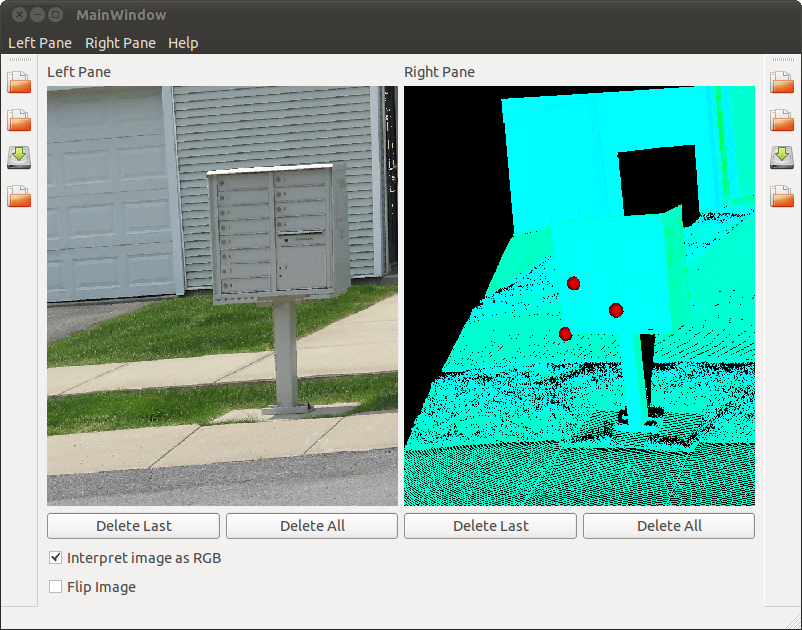
\includegraphics[width=0.6\linewidth]{images/PointCloudZoomedOut}
    \caption{Screenshot of a zoomed out view of point cloud correspondences}
    \label{fig:PointCloudZoomedOut}
  \end{figure}
\end{center} 

When zoomed in, the text indicates the number of the point, as shown in Figure \ref{fig:PointCloudZoomedIn}. The sphere has the radius of the average distance between points in the data set in an attempt to always make the sphere useful and unintrusive, no matter the scale of the data set.

\begin{center}
  \begin{figure}[H]
  \centering
    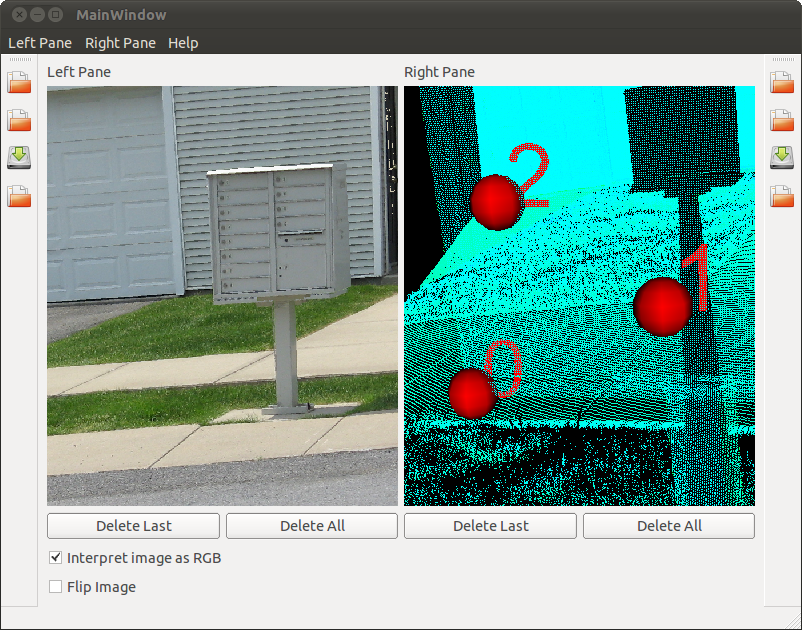
\includegraphics[width=0.6\linewidth]{images/PointCloudZoomedIn}
    \caption{Screenshot of a zoomed in view of point cloud correspondences}
    \label{fig:PointCloudZoomedIn}
  \end{figure}
\end{center} 

In the example you will notice that the point cloud is pseudo-colored. In this application, we are finding correspondences between an image and a LiDAR scan which will be used to compute the projection matrix between the data sets so that we can re-color the LiDAR points with the image colors. The pseudo-coloring of the points encodes their return intensity, which makes it possible to differentiate different materials, making it much easier to identify and select appropriate correspondences. If the points were all colored with the same color, it is very hard to identify such correspondences.

%%%%%%%%%%%%%%%%
\section{Saving and Loading Correspondences}
We use a simple plain text format for saving and loading correspondences. Each correspondence is written to a line of a text file, with its coordinates space-delimited. An example image correspondence file with 4 correspondences looks like this:
\begin{verbatim}
1433 729
1716 733
1434 1023
1712 1031
\end{verbatim}

while a point cloud correspondence file is similar but with a 3rd coordinate:

\begin{verbatim}
-0.279922 15.4904 0.122696
0.45491 15.2637 0.162918
0.582443 15.6512 0.170822
-0.253708 15.5121 -0.662094
\end{verbatim}

Once correspondences are selected, they can be saved using the ``Save points'' button on the corresponding pane's toolbar, or the ``Save points'' file menu option from the corresponding pane's file menu.

When correspondences are loaded from a file, they are added to the pane exactly as if the user had selected them during this session.


\end{document}